\documentclass[11pt,a4paper]{article}
\usepackage[utf8]{inputenc}
\usepackage[spanish]{babel}	%Idioma
\usepackage{amsmath}
\usepackage{amsfonts}
\usepackage{amssymb}
\usepackage{graphicx} 	%Añadir imágenes
\usepackage{geometry}	%Ajustar márgenes
\usepackage[export]{adjustbox}[2011/08/13]
\usepackage{float}
\restylefloat{table}
\usepackage[hidelinks]{hyperref}
\usepackage{titling}
\graphicspath{{/home/nazaret/Escritorio/LaTEX}}
%\usepackage{minted}
\usepackage{multirow}
\usepackage{caption}
\usepackage{multicol}
\usepackage[shortlabels]{enumitem}
\usepackage{array}
\selectlanguage{spanish}

%Opciones de encabezado y pie de página:
\usepackage{fancyhdr}
\pagestyle{fancy}
\lhead{Nazaret Román Guerrero}
\rhead{Redes Multiservicio}
\lfoot{Grado en Ingeniería Informática}
\cfoot{}
\rfoot{\thepage}
\renewcommand{\headrulewidth}{0.4pt}
\renewcommand{\footrulewidth}{0.4pt}

%Opciones de fuente:
\usepackage[utf8]{inputenc}
\usepackage[default]{sourcesanspro}
\usepackage{sourcecodepro}
\usepackage[T1]{fontenc}

\setlength{\parindent}{15pt}
\setlength{\headheight}{15pt}
\setlength{\voffset}{10mm}

% Custom colors
\usepackage{color}
\definecolor{deepblue}{rgb}{0,0,0.5}
\definecolor{deepred}{rgb}{0.6,0,0}
\definecolor{deepgreen}{rgb}{0,0.5,0}

\usepackage{xcolor}
\usepackage{listings}
\lstset{basicstyle=\ttfamily, basicstyle=\footnotesize,
  showstringspaces=false,
  commentstyle=\color{red},
  keywordstyle=\color{blue}
}

\begin{document}
\begin{titlepage}

\begin{minipage}{\textwidth}

\centering

\includegraphics[width=0.6\textwidth]{img/logo.png}\\

\textsc{\Large Redes Multiservicio\\[0.2cm]}
\textsc{GRADO EN INGENIERÍA INFORMÁTICA}\\[1cm]

{\Huge\bfseries Configuración de \textit{shaping} en VyOS\\}
\noindent\rule[-1ex]{\textwidth}{3pt}\\[3.5ex]
{\large\bfseries Tarea 3}
\end{minipage}

\vspace{1cm}
\begin{minipage}{\textwidth}
\centering

\textbf{Autores}\\ {Pedro Parrilla Navarro\\ Nazaret Román Guerrero}\\[2.5ex]

\includegraphics[width=0.35\textwidth]{img/etsiit.jpeg}\\[0.1cm]
\vspace{0.5cm}
\textsc{Escuela Técnica Superior de Ingenierías Informática y de Telecomunicación}\\
\vspace{0.5cm}
\textsc{Curso 2018-2019}
\end{minipage}
\end{titlepage}

\pagenumbering{gobble}
\pagenumbering{arabic}

\newpage

\section{Configuración del \textit{shaping} en VyOS}

\subsection{Instalación de \textit{VyOS}}

Lo primero es llevar a cabo la instalación del sistema operativo del \textit{router}. Para ello hemos descargado un \texttt{.iso} de \color{blue}\url{https://www.vyos.io/rolling-release/}\color{black}.\\

Utilizando \textit{VirtualBox} hemos instalado el sistema, tal y como se puede ver en las siguientes imágenes.

\begin{figure}[H]
	\centering
	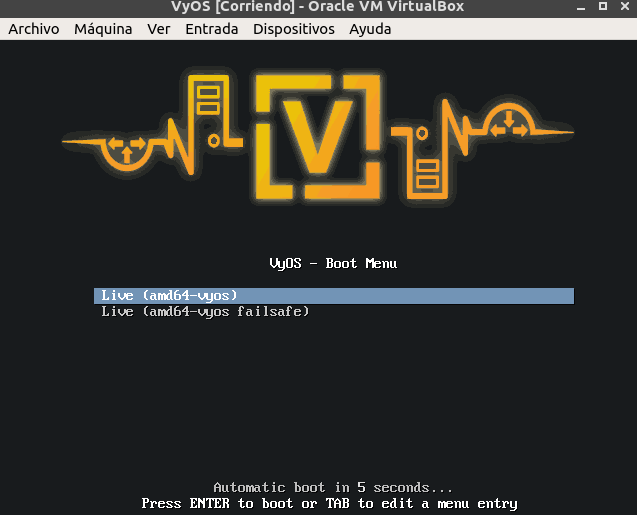
\includegraphics[scale=0.35]{img/init.png}
	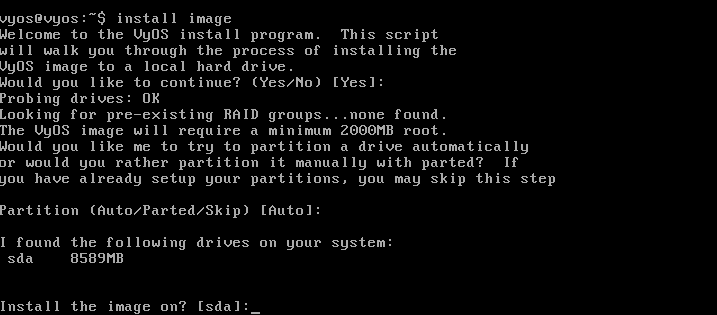
\includegraphics[scale=0.32]{img/instalacion-imagen.png}
\end{figure}

Como cualquier instalación, nos pregunta sobre el disco que se acaba de crear. Aceptamos que se elimine y hemos terminado la instalación. El usuario y la contraseña son \textit{vyos}.

\begin{figure}[H]
	\centering
	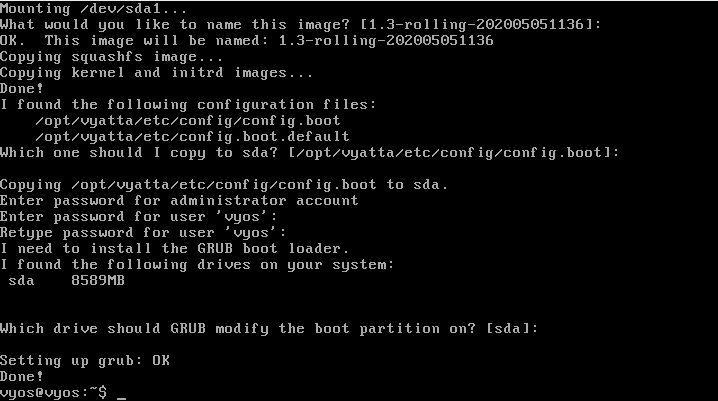
\includegraphics[scale=0.3]{img/sda-fin.png}
\end{figure}

\subsection{Configuración de la interfaz \texttt{eth0}}

La configuración inicial de las interfaces de red la podemos ver con el comando:\\

\begin{lstlisting}[language=bash]
$ show interfaces
\end{lstlisting}

\vspace{0.3cm} La salida del comando antes de configurarla es la que sigue:

\begin{figure}[H]
	\centering
	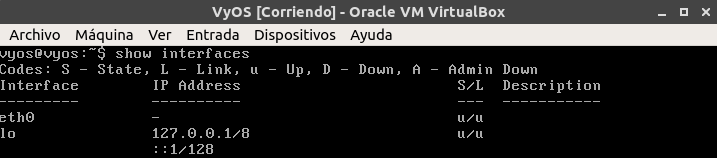
\includegraphics[scale=0.5]{img/show-init-interfaces.png}
\end{figure}

Como podemos ver, hay dos interfaces, \texttt{eth0}, que no está configurada, y el \textit{loopback}. Así que vamos a configurar la interfaz y después impondremos una política de \textit{shaping}. Para ello, debemos entrar la modo de configuración mediante el comando \texttt{configure} (saldrá un símbolo \#, similar a los \textit{routers} Cisco), y configurar la interfaz usando\\

\begin{lstlisting}[language=bash]
$ set interfaces ethernet eth0 address 10.0.0.1/24
\end{lstlisting}

\vspace{0.3cm} Tras configurarla debemos ejecutar \texttt{commit} para actualizar los cambios y que se guarden. Una vez que lo hemos hecho, mostramos la configuración de nuevo. El proceso se puede ver en la imagen siguiente.

\begin{figure}[H]
	\centering
	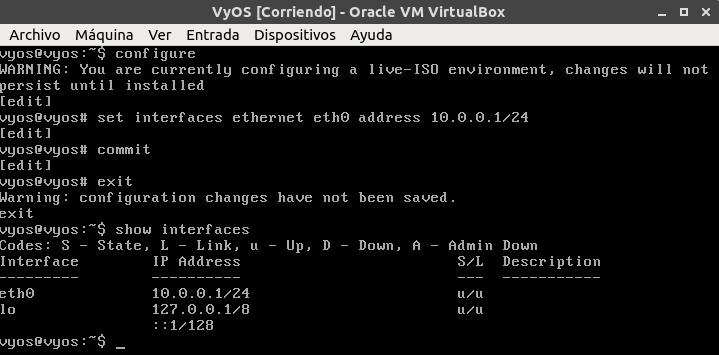
\includegraphics[scale=0.5]{img/show-interfaces-fin.png}
\end{figure}

Como podemos ver la interfaz está levantada (\texttt{S/L = u/u}), por lo que está en funcionamiento. Una vez hecho esto, vamos a configurar el \textit{shaping}.

\newpage

\subsection{Configuración del \textit{shaping}}

Configurar el \textit{shaping} es sencillo: necesitamos crear una política con un nombre e indicar los parámetros que desamos. Se puede añadir una descripción también aunque nosotros no lo hemos hecho.\\

Nosotros vamos a crear una política llamada \texttt{SHAPINGRMS} en la que vamos a establecer una tasa de 50 kbps, tal y como se puede ver en la imagen siguiente:

\begin{figure}[H]
	\centering
	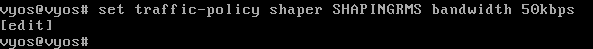
\includegraphics[scale=0.5]{img/shaping.png}
\end{figure}

Tras crear la política, debemos asignarla a una interfaz. Como solo tenemos una política ahora mismo, no hace falta indicar a cuál se le aplica a la interfaz. Lo vamos a aplicar a la entrada y la salida de paquetes de \texttt{eth0}. Podemos ver el procedimiento en la imagen siguiente:

\begin{figure}[H]
	\centering
	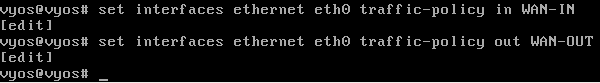
\includegraphics[scale=0.5]{img/shaping-en-interface.png}
\end{figure}

Para comprobar que se ha aplicado la política en la interfaz, utilizamos de nuevo el comando \texttt{show interfaces}. La salida es la siguiente:

\begin{figure}[H]
	\centering
	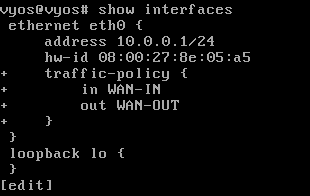
\includegraphics[scale=0.5]{img/config-con-shape.png}
\end{figure}

Por lo que podemos ver, la configuración está aplicada correctamente a la interfaz. Ahora solo nos queda probarla.

\newpage

\section{Pruebas con ITG y wireshark}

Para comprobar el funcionamiento y ver el gráfico de entrada y salida vamos a utilizar ITG para generar el tráfico y wireshark para capturarlo y poder extraerlo.\\

Para generar el tráfico usamos la siguiente orden que ya hemos usado en la práctica 1. El tráfico es de VoIP y está dirigido al router a través del puerto 4444. El envío de paquetes se produce durante 2 segundos.

\begin{figure}[H]
	\centering
	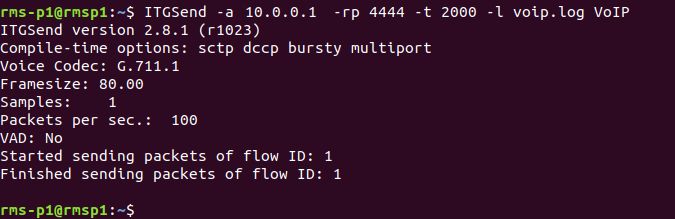
\includegraphics[scale=0.5]{img/itg.png}
\end{figure}

Puesto que se han capturado muchos paquetes (un total de 172 paquetes), hemos puesto aquí solo un fragmento de la captura que hemos cogido:

\begin{table}[H]
\centering
\begin{tabular}{|c|c|c|c|c|c|}
\hline
\textbf{No.}  & \textbf{Time}        & \textbf{Source}    & \textbf{Destination} & \textbf{Protocol} & \textbf{Length} \\ \hline
30  & 0.713997675 & 192.168.1.132 & 10.0.0.1   & UDP      & 116    \\ \hline
31  & 0.714023341 & 192.168.1.132 & 10.0.0.1   & UDP      & 102    \\ \hline
32  & 0.714051516 & 192.168.1.132 & 10.0.0.1   & UDP      & 112    \\ \hline
33  & 0.714059899 & 192.168.1.132 & 10.0.0.1   & UDP      & 111    \\ \hline
34  & 0.714090366 & 192.168.1.132 & 10.0.0.1   & UDP      & 107     \\ \hline
35  & 0.770107081 & 192.168.1.132 & 10.0.0.1   & UDP      & 117    \\ \hline
36  & 0.770620425 & 192.168.1.132 & 10.0.0.1   & UDP      & 103    \\ \hline
37  & 0.770654958 & 192.168.1.132 & 10.0.0.1   & UDP      & 122    \\ \hline
38 & 0.773119827 & 192.168.1.132 & 10.0.0.1   & UDP      & 106    \\ \hline
39 & 0.804828754 & 192.168.1.132 & 10.0.0.1   & UDP      & 106    \\ \hline
40 & 0.804842598 & 192.168.1.132 & 10.0.0.1   & UDP      & 107     \\ \hline
41 & 0.804897625 & 192.168.1.132 & 10.0.0.1   & UDP      & 121    \\ \hline
42 & 0.807561982 & 192.168.1.132 & 10.0.0.1   & UDP      & 106     \\ \hline
43 & 0.808932682 & 192.168.1.132 & 10.0.0.1   & UDP      & 103    \\ \hline
44 & 0.808962465 & 192.168.1.132 & 10.0.0.1   & UDP      & 99    \\ \hline
\end{tabular}
\caption{Fragmento de captura}
\end{table}

Todos los paquetes enviado se reciben en el router, pero cuando este llega al límite impuesto (50 kbps), frena la llegada de paquetes para no saturarse.\\

Con wireshark hemos sacado el gráfico de entrada/salida, es el siguiente:

\begin{figure}[H]
	\centering
	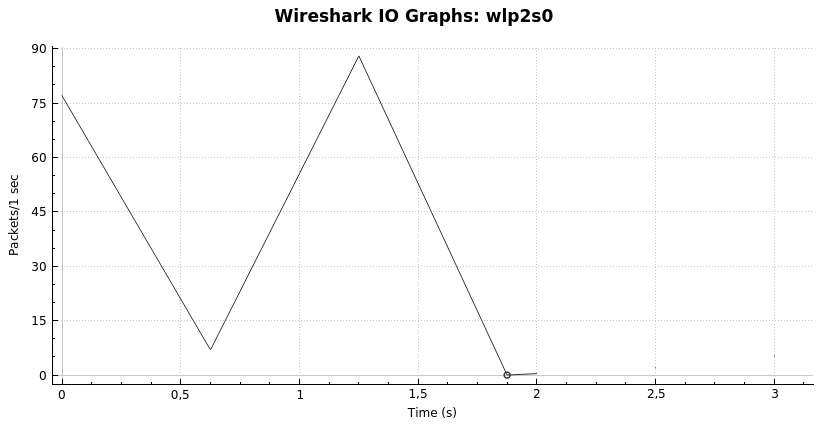
\includegraphics[scale=0.5]{img/iostat.png}
\end{figure}

Como podemos ver hay dos picos donde se mandan muchos paquetes e inmediatamente el pico disminuye casi a 0: el \textit{router} ha alcanzado su límite y frena la llegada de paquetes para no saturarse. El gráfico es muy visual en ese aspecto y es fácil observar que el \textit{shaping} está frenando la entrada de más paquetes al \textit{router}. Por tanto la política de \textit{shaping} que hemos configurado está funcionado correctamente.

\section{Bibliografía}

\begin{itemize}
	\item \color{blue} \url{https://wiki.vyos.net/wiki/Basic_setup}\color{black}
	\item \color{blue} \url{https://wiki.vyos.net/wiki/QoS#interface}
\end{itemize}

\end{document}